\documentclass[a4paper]{article}
\usepackage{ucs}
\usepackage[utf8x]{inputenc}
\usepackage[T1]{fontenc}
\usepackage{german}
\usepackage{a4,ngerman}
\usepackage[ngerman]{babel}
\usepackage{graphicx}
\usepackage[]{cite}
\usepackage{fancyhdr}
\usepackage{amsmath}
\pagestyle{fancy}
\selectlanguage{german}
\usepackage{array}
\usepackage{mathtools}
\cfoot{\textcopyright Lukas Schörghuber, S1610307103}

\begin{document}
	\begin{enumerate}
		\item
		\begin{enumerate}
			\item
			\begin{equation*}
				(\lnot x \lor y) \lor ((y \land x) \lor (y \land z))
			\end{equation*}
			\begin{equation*}
				\lnot x \lor y \lor (y \land z) \lor (y \land x)
			\end{equation*}
			\begin{equation*}
				\lnot x \lor y \lor (y \land x)
			\end{equation*}
			\begin{equation*}
				\lnot x \lor y
			\end{equation*}
			\begin{equation*}
				x \Rightarrow y
			\end{equation*}
			
			\item
			\begin{equation*}
				((A \lor \lnot B) \land (A \lor A)) \land (A \lor B \lor C)
			\end{equation*}
			\begin{equation*}
				((A \lor \lnot B) \land A) \land (A \lor (B \lor C))
			\end{equation*}
			\begin{equation*}
				A \land (A \lor (B \lor C))
			\end{equation*}
			\begin{equation*}
				(A \land A) \lor (A \land (B \lor C))
			\end{equation*}
			\begin{equation*}
				A \lor ((A \land B) \lor (A \land C))
			\end{equation*}
			\begin{equation*}
				(A \lor (A \land B)) \lor (A \land C)
			\end{equation*}
			\begin{equation*}
				A \lor (A \land C)
			\end{equation*}
			\begin{equation*}
				A
			\end{equation*}
		\end{enumerate}
		
		\item
		\begin{enumerate}
			\item
			\begin{equation*}
				(\lnot x \land \lnot y) \lor (x \lor (x \land y))
			\end{equation*}
			\begin{equation*}
				(\lnot x \land \lnot y) \lor x
			\end{equation*}
			\begin{equation*}
				(\lnot x \lor x) \land (\lnot y \lor x)
			\end{equation*}
			\begin{equation*}
				w \land (\lnot y \lor x)
			\end{equation*}
			\begin{equation*}
				\lnot y \lor x
			\end{equation*}
			\begin{equation*}
				y \Rightarrow x
			\end{equation*}
			
			\item
			\begin{equation*}
				((x \lor \lnot x) \land (x \lor y)) \land ((x \lor x) \land (x \lor y))
			\end{equation*}
			\begin{equation*}
				(w \land (x \lor y)) \land (x \land (x \lor y))
			\end{equation*}
			\begin{equation*}
				(x \lor y) \land x
			\end{equation*}
			\begin{equation*}
				x
			\end{equation*}
		\end{enumerate}
		
		\item
		\begin{enumerate}
			\item
			\begin{equation*}
				(A \otimes B) \land B
			\end{equation*}
			\newline
			Alternative:
			\begin{equation*}
				\lnot A \land B
			\end{equation*}
			
			\item
			\begin{equation*}
				(\lnot A \land \lnot B \land C) \lor (\land A \land B \land C) \lor (A \land B \land \lnot C)
			\end{equation*}
		\end{enumerate}
		\clearpage
		
		\item
		\begin{enumerate}
			\item
			\begin{equation*}
				\underbrace{f(\underbrace{-(\underbrace{+(\underbrace{*(\underbrace{x}_{\text{Term}}, \underbrace{2}_{\text{Term}})}_{\text{Term}}, \underbrace{y}_{\text{Term}}}_{\text{Term}}), \underbrace{2}_{\text{Term}})}_{\text{Term}}, \underbrace{+(\underbrace{2}_{\text{Term}}, \underbrace{x}_{\text{Term}})}_{\text{Term}}, \underbrace{\leq(\underbrace{4}_{\text{Term}}, \underbrace{3}_{\text{Term}})}_{\text{atomare Aussage}})}_{\text{ungültig, da einer der drei Eingabeparameter eine a.A. ist}}
			\end{equation*}
			
			\item
			\begin{equation*}
				\underbrace{P(\underbrace{+(\underbrace{2}_{\text{Term}}, \underbrace{3}_{\text{Term}})}_{\text{Term}}, \underbrace{f(\underbrace{1}_{\text{Term}}, \underbrace{2}_{\text{Term}}, \underbrace{x}_{\text{Term}})}_{\text{Term}})}_{\text{atomare Aussage}}
			\end{equation*}
			
			\item
			\begin{equation*}
				\underbrace{/(\underbrace{f(\underbrace{2}_{\text{Term}}, \underbrace{3}_{\text{Term}}, \underbrace{4}_{\text{Term}})}_{\text{Term}}, \underbrace{-(\underbrace{x}_{\text{Term}}, \underbrace{y}_{\text{Term}})}_{\text{Term}}))}_{\text{Term}}
			\end{equation*}
			
			\item
			\begin{equation*}
				\underbrace{\leq(\underbrace{Q(\underbrace{*(\underbrace{2}_{\text{Term}}, \underbrace{4}_{\text{Term}})}_{\text{Term}}, \underbrace{P(\underbrace{13}_{\text{Term}}, \underbrace{x}_{\text{Term}})}_{\text{atomare Aussage}})}_{\text{ungültig, da Eingabe Term und a.A.}}, \underbrace{f(\underbrace{x}_{\text{Term}}, \underbrace{2}_{\text{Term}}, \underbrace{3}_{\text{Term}})}_{\text{Term}})}_{\text{ungültig, da Eingabe Term und atomare Aussage}}
			\end{equation*}
			
			\item
			\begin{equation*}
				\underbrace{+(\underbrace{2}_{\text{Term}}, \underbrace{*(\underbrace{3}_{\text{Term}}, \underbrace{x}_{\text{Term}})}_{\text{Term}}, \underbrace{-(\underbrace{3}_{\text{Term}}, \underbrace{9}_{\text{Term}})}_{\text{Term}})}_{\text{ungültig, da + nur eine zweistellige Funktionskonstante ist}}
			\end{equation*}
			
			\item
			\begin{equation*}
				\underbrace{+(\underbrace{P(\underbrace{3}_{\text{Term}}, \underbrace{x}_{\text{Term}})}_{\text{atomare Aussage}}, \underbrace{-(\underbrace{2}_{\text{Term}}, \underbrace{y}_{\text{Term}})}_{\text{Term}})}_{\text{ungültig, da Eingabe a.A. und Term}}
			\end{equation*}
		\end{enumerate}
		\clearpage
		
		\item
		\begin{enumerate}
			\item
			\begin{equation*}
				\begin{aligned}
					( \underbrace{f((\underbrace{x}_{\text{V}}, ( \underbrace{x}_{\text{V}} \underbrace{*}_{\text{FK2}} \underbrace{2}_{\text{OK}} ), \underbrace{2}_{\text{OK}})}_{\text{FK3}} \underbrace{-}_{\text{FK2}} ( \underbrace{2}_{\text{OK}} \underbrace{+}_{\text{FK2}} \underbrace{x}_{\text{V}})\underbrace{\leq}_{\text{PK}} ( \underbrace{4}_{\text{OK}} \underbrace{/}_{\text{FK2}} \underbrace{x}_{\text{V}} )) \\ \Rightarrow \\ (((\underbrace{4}_{\text{OK}} \underbrace{-}_{\text{FK2}} \underbrace{x}_{\text{V}}) \underbrace{<}_{\text{PK2}} (\underbrace{5}_{\text{OK}} \underbrace{+}_{\text{FK2}} \underbrace{x}_{\text{V}})) \land \underbrace{P(\underbrace{3}_{\text{OK}}, (\underbrace{x}_{\text{V}} \underbrace{/}_{\text{FK2}} \underbrace{y}_{\text{V}}))}_{\text{PK2}})
				\end{aligned}
			\end{equation*}
			\begin{figure}[ht!]
				\begin{center}
					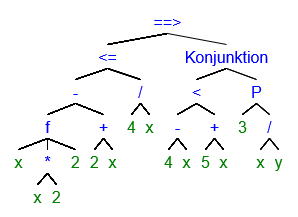
\includegraphics[height=45mm]{5a.png}
					\caption{Syntaxbaum für Aufgabe 5)a)}
				\end{center}
			\end{figure}
		
			\item
			\begin{equation*}
				\begin{aligned}
					(\underbrace{f(\underbrace{z}_{\text{V}}, (\underbrace{x}_{\text{V}} \underbrace{+}_{\text{FK2}} \underbrace{2}_{\text{OK}}), (\underbrace{y}_{\text{V}} \underbrace{-}_{\text{FK2}} \underbrace{2}_{\text{OK}}))}_{\text{FK3}} \underbrace{-}_{\text{FK2}} (\underbrace{3}_{\text{OK}} \underbrace{/}_{\text{FK2}} \underbrace{z}_{\text{V}})) \\ \underbrace{/}_{\text{FK2}} \\ ((\underbrace{3}_{\text{OK}} \underbrace{*}_{\text{FK2}} (\underbrace{x}_{\text{V}} \underbrace{*}_{\text{FK2}} \underbrace{y}_{\text{V}})) \underbrace{-}_{\text{FK2}} (\underbrace{4}_{\text{OK}} \underbrace{*}_{\text{FK2}} \underbrace{z}_{\text{V}}))
				\end{aligned}
			\end{equation*}
			\begin{figure}[ht!]
				\begin{center}
					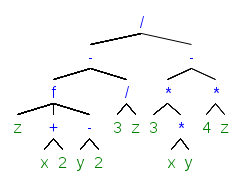
\includegraphics[height=45mm]{5b.png}
					\caption{Syntaxbaum für Aufgabe 5)b)}
				\end{center}
			\end{figure}
		\end{enumerate}
		
	\end{enumerate}
\end{document}